\chapter{Linear Models}
\label{linear-models}

Regression Analysis represents a set of statistical methods and techniques, which we use to evaluate the relationship between variables. These are one dependent variable (our target) and one or more independent variables (predictors).

We have three primary variants of regression — simple linear, multiple linear, and non-linear. However, most of the time, we use linear regression models. Non-linear models are helpful when working with more complex data, where variables impact each other in a non-linear way.

Regression Analysis has many applications, and one of the most common is in financial analysis and modeling.

In financial modeling, we can employ regression analysis to estimate the strength of the relationship between variables and subsequently forecast this relationship’s future behavior. It fits in any setting where we hypothesize there is (or not) a correlation between two or more variables.

\section{Simple Linear Regression Analysis}
\label{sec:linear-regression}
Regression Analysis is a form of predictive analysis. It can be used to find the relation of a company’s performance to the industry performance or competitor business.

The single (or simple) linear regression model expresses the relationship between the dependent variable (target) and one independent variable. Regression attempts to find the strength of that relationship.

We use it to analyze the statistical relationship between sets of variables. Regression models usually show a regression equation representing the dependent variable as a function of the independent variable.
A simple linear model can be described by the following equation:
\begin{equation}
y = \beta x + \alpha + \epsilon
\label{eq:linear_regression}
\end{equation}
where $y$ is the dependent variable (the target), $\alpha$ the intercept, $\beta$ the slope, $x$ the independent variable (the predictor), and $\epsilon$ the residual (error).

The purpose is to estimate the underlying relationship so that we can predict the target variable based on the other (predictor).

%We can plot the function on a graph, where a is the intercept and b is the slope. It shows us the measure of the change in the target variable due to changes in other variables. We can use it when we attempt to identify the variables that affect a certain measure, like a stock price.

\subsection{Ordinary Least Squares}
We need to solve a problem when running the regression model, and this is to fit a straight line to a set of pairs of observations of the dependent and independent variables. The line of best fit is where the sum of the squares of the vertical deviations (distances) between observation points and the line is at its minimum. This is the method of ordinary least squares (OLS) and the one we most commonly apply to a linear regression model.

\begin{figure}[htbp]
\centering
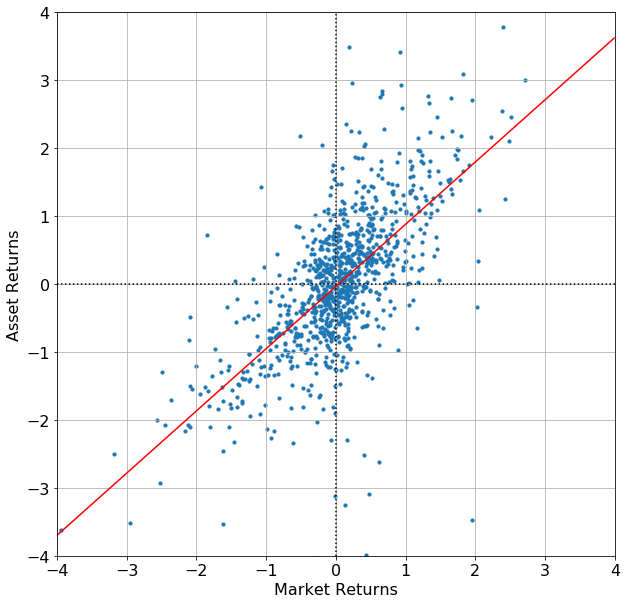
\includegraphics[width=0.7\textwidth]{figures/linear_regression}
\caption{Example of linear regression.}
\label{fig:linear_regression_example}
\end{figure}

The regression equation gives no exact prediction of the target value for any predictor variable. The regression coefficients we calculate from our sample data observations are only the best estimate of the real population variables.
This is why we introduce $\epsilon$ (residual/error) to the model, it covers the element of chance that an independent variable can experience variations.

\subsubsection{Covariance}
One of the measures we get from a regression analysis is the covariance. It calculates the relationship between two variables.

\begin{equation}
\textrm{cov}(x, y) = \mathbb{E}[(x - \mathbb{E}[x])(y - \mathbb{E}[y])]
\end{equation}
where: $x$ and $y$ are the values of the independent and dependent variables at each observation, and $\mathbb{E}$ represents the mean.

The formula shows the direction of the relationship. If one variable is going up when the other is going down, then the covariance will be negative, and vice versa.

\subsubsection{Correlation}
That’s where correlation, another measure of regression analysis, comes in. It helps us to standardize the covariance to be able to better understand and use it in forecasting.

Correlation takes the covariance and divides it over the product of the standard deviations of the variables. This makes sure we get a correlation coefficient between -1 and +1.
\begin{equation}
\textrm{cor}(x, y) = \frac{\textrm{cov}(x, y)}{\textrm{std}(x)\textrm{std}(y)}
\end{equation}

A correlation of +1 suggests the two variables are perfectly positively correlated, and a value of -1 suggests an entirely negative correlation.

From the definition of the $\beta$ coefficient (i.e. the slope of the linear regression) through least squares we have
\begin{equation}
\hat{\beta} = \textrm{cor}(x, y)\cdot \frac{\textrm{std}(y)}{\textrm{std}(x)}
\end{equation}
therefore the two only coincide when $\textrm{std}(y) = \textrm{std}(x)$ That is, they only coincide when the two variables are, in some sense, on the same scale. 

Correlation and slope at some extent give the same information, i.e. they each tell the linear relationship strength between $x$ and $y$. But, they also do each give distinct information:
\begin{itemize}
\item the correlation gives you a bounded measurement that can be interpreted independently of the two variables scale. The closer the estimated correlation is to $\pm1$, the closer the two are to a perfect linear relationship. The regression slope, in isolation, does not tell you that piece of information.
\item the regression slope gives a useful quantity interpreted as the estimated change in the expected value of $y$ for a given value of $x$. Specifically, $\hat{\beta}$ tells you the change in the expected value of $y$ corresponding to a 1-unit increase in $x$. This information can not be deduced from the correlation coefficient alone.
\end{itemize}

%Model Assumptions
%Whenever we are setting up a regression model, we need to work with some inherent assumptions. The most notable amongst those are:
%
%The variables exhibit a linear relationship between the slope and intercept;
%The independent variable (predictor) is not random;
%The values of the residuals (errors) follow a standard normal distribution.

\subsection{Multiple Linear Regression}
Simple regression is usually not enough in a real-life scenario, as targets (dependent variables) are rarely impacted only by a single predictor.
The multiple linear regression model is almost the same as the simple one; the only difference being it can have two or more independent variables (predictors).
The function to represent the regression equation is:
\begin{equation}
y = \beta_1 x_1 + \beta_2 x_2 + \ldots + \beta_n x_n + \alpha + \epsilon
\label{eq:multiple_regression}
\end{equation}

It is crucial to keep in mind that the multiple regression model requires \emph{non-collinearity}. This means the independent variables should have a minimal correlation between them. Otherwise, it is difficult to assess the real relationship between the dependent (target) and the independent (predictors) variables.

\subsection{Linear Regression Example}

The Chinese Yuan (CNY) was pegged to the US Dollar (USD) prior to July 2005. Then, China announced that the exchange rate would be set with reference to a basket of other currencies, allowing for a movement of up to 0.3\% within any given day. The actual currencies and their basket weights are unannounced by China. Figure~\ref{fig:yuan_rate} reports the Yuan exchange rate to USD between 1999 and 2013.

\begin{figure}[htbp]
\centering
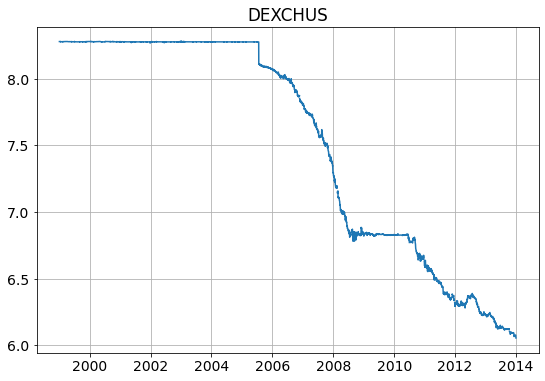
\includegraphics[width=0.7\textwidth]{figures/yuan_exchange_rate}
\caption{Yuan exchange rate to USD from January 1999 to December 2013.}
\label{fig:yuan_rate}
\end{figure}

From an empirical point of view, there are several important questions:
\begin{itemize}
\item for any given period, what is the implicit reference basket for the Chinese currency ?
\item has the reference basket changed over time ?
\item has the Chinese currency depreciated with respect to the dollar? If so, how much and when?
\end{itemize}

A possible approach for evaluating the implicit exchange rate regime of the Yuan involves the regression of the changes in the target currency on changes in the values of possible currencies in the reference basket.

Consider the dataset \href{https://raw.githubusercontent.com/matteosan1/finance_course/develop/libro/input_files/exchange_rates.csv}{exchange\_rates.csv} containing daily currencies exchange rates in the 1999 to 2013 period (data has been fetched from the Federal Reserve Archive~\cite{bib:fred}).

To apply this methodology the original dollar-based exchange rates have been converted using the Swiss Franc. This allows currency moves of the dollar to be be used to explain moves in the Yuan. The choice of Swiss Franc is consistent with evaluations with respect to a stable currency. The dataframe already has columns with daily variations.

\begin{ipython}
import pandas as pd

data = pd.read_csv("exchange_rates.csv", index_col="Date")
print (data.head())
\end{ipython}
\begin{ioutput}
            DEXCHUS  DEXJPUS  DEXKOUS  DEXMAUS  DEXUSEU  DEXUSUK  DEXTHUS  \
Date                                                                        
1999-01-05   8.2795   111.15   1166.0      3.8   1.1760   1.6566    36.18   
1999-01-06   8.2795   112.78   1160.0      3.8   1.1636   1.6547    36.50   
1999-01-07   8.2798   111.69   1151.0      3.8   1.1672   1.6495    36.30   
1999-01-08   8.2796   111.52   1174.0      3.8   1.1554   1.6405    36.45   
...
                ret_THB_SFR      ret_USD_SFR  
Date                                          
1999-01-05        -0.002599        -0.002047  
1999-01-06        -0.002666        -0.011472  
1999-01-07        -0.006288        -0.000794  
1999-01-08        -0.003565        -0.007689  

[5 rows x 24 columns]
\end{ioutput}

%Figure~\ref{fig:rate_variation} shows CNY and USD daily variation with respect to Swiss Franc (SFR).
%\begin{figure}[htbp]
%\centering
%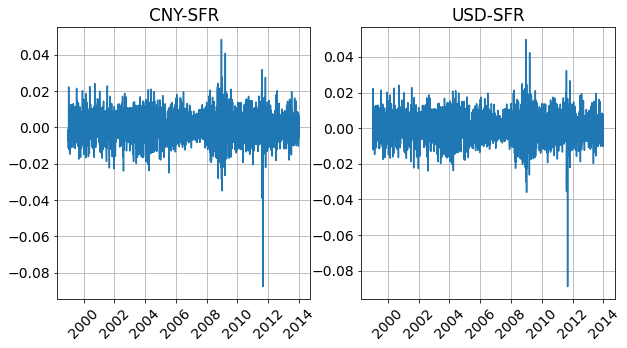
\includegraphics[width=0.7\textwidth]{figures/log_variation_exch}
%\caption{Daily variation of CNY and USD exchange rates from January 1999 to December 2013 with respect to Swiss Franc.}
%\label{fig:rate_variation}
%\end{figure}

To implement the linear regression model it can be used the \texttt{statsmodel} package. It is necessary to define the $X$ vector (i.e. the independent exchange rate variations) and $y$ (i.e. the target Yuan rate to SFR). Then add a constant to the model which represents the rate variation not correlated to other currency variations (i.e. $\alpha$).

First, we fit the regression model for the period prior to July 2005 when the Chinese currency was pegged to the US dollar. 

\begin{ipython}
import statsmodels.api as sm

X = df.loc[df.index < '2005-06-30' ,
           ['ret_YEN_SFR', 'ret_EUR_SFR', 
            'ret_GBP_SFR', 'ret_USD_SFR']]
y = df.loc[df.index < '2005-06-30' ,'ret_CNY_SFR']
X = sm.add_constant(X)

est = sm.OLS(y, X).fit()
print(est.summary())
\end{ipython} 
\begin{ioutput}
                            OLS Regression Results                            
==============================================================================
Dep. Variable:            ret_CNY_SFR   R-squared:                       1.000
Model:                            OLS   Adj. R-squared:                  1.000
Method:                 Least Squares   F-statistic:                 3.647e+06
Date:                Tue, 08 Nov 2022   Prob (F-statistic):               0.00
Time:                        13:46:53   Log-Likelihood:                 13749.
No. Observations:                1692   AIC:                        -2.749e+04
Df Residuals:                    1687   BIC:                        -2.746e+04
Df Model:                           4                                         
Covariance Type:            nonrobust                                         
===============================================================================
                  coef    std err          t      P>|t|      [0.025      0.975]
-------------------------------------------------------------------------------
const       -1.921e-07   1.74e-06     -0.110      0.912   -3.61e-06    3.23e-06
ret_YEN_SFR    -0.0001      0.000     -0.477      0.633      -0.001       0.000
ret_EUR_SFR    -0.0003      0.001     -0.379      0.705      -0.002       0.001
ret_GBP_SFR    -0.0001      0.000     -0.224      0.823      -0.001       0.001
ret_USD_SFR     1.0002      0.000   2545.320      0.000       0.999       1.001
==============================================================================
Omnibus:                      758.491   Durbin-Watson:                   2.824
Prob(Omnibus):                  0.000   Jarque-Bera (JB):           889538.472
Skew:                           0.456   Prob(JB):                         0.00
Kurtosis:                     115.324   Cond. No.                         486.
==============================================================================
\end{ioutput} 

The most interesting (for us) part of the summary is: 
\begin{itemize}
\item R-squared: the closer to 1 the higher is the linear correlation between $y$ and $X$;
\item coef: the estimate of this model parameter (the weight assigned to this feature);
\item std err: the standard error of our estimate. From these two values we can compute the t-score of our estimate:
\begin{equation*}
t = \frac{\textrm{coeff}}{\textrm{std err}}
\end{equation*}
which we can find on the third column ($t$); 
\item t: this value essentially provides us with a metric of how small the error is with respect to the estimated value: the larger the t-score, the smaller the error and the more confident we can be in our estimate.
\item P>|t|: to better quantify our confidence, it’s usual to compute the p-value associated to the t-score. Under relatively common assumptions, we expect the t-score to follow a standard distribution and the probability of obtaining results at least as extreme as the value observed is simply the area under the curve to the right of the t-score value. This area is known as the p-value.
There are some nuances to interpreting p-values but briefly, the smaller the p-value, the stronger the evidence that the value we’re estimating is different than zero (if the coefficient of a given feature is indistinguishable from zero then that feature is not relevant for our model).

Typical thresholds for the p-value are:
\begin{itemize}
	\item $p<0.05$: moderate evidence;
	\item $p<0.01$: strong evidence;
	\item $p<0.001$: very strong evidence.
\end{itemize}
\end{itemize}

In our example R-squared is 1, and the only largely significant predictor is USD (p-value 0) confirming that indeed CNY was anchored to US dollar prior July 2005.

Second, we fit the regression model for the first six months following the announcement of the change in currency policy.

\begin{ipython}
X = df.loc[(df.index > '2005-07-01') & (df.index < '2005-12-31'),
           ['ret_YEN_SFR', 'ret_EUR_SFR', 
            'ret_GBP_SFR', 'ret_USD_SFR',
            'ret_WON_SFR', 'ret_MYR_SFR', 
            'ret_THB_SFR']]
y = df.loc[(df.index > '2005-07-01') & (df.index < '2005-12-31'),
           'ret_CNY_SFR']

X = sm.add_constant(X)
est = sm.OLS(y, X).fit()
print(est.summary())
\end{ipython}
\begin{ioutput}
                            OLS Regression Results                            
==============================================================================
Dep. Variable:            ret_CNY_SFR   R-squared:                       0.949
Model:                            OLS   Adj. R-squared:                  0.946
Method:                 Least Squares   F-statistic:                     326.3
Date:                Tue, 08 Nov 2022   Prob (F-statistic):           8.41e-76
Time:                        13:53:28   Log-Likelihood:                 667.58
No. Observations:                 130   AIC:                            -1319.
Df Residuals:                     122   BIC:                            -1296.
Df Model:                           7                                         
Covariance Type:            nonrobust                                         
===============================================================================
                  coef    std err          t      P>|t|      [0.025      0.975]
-------------------------------------------------------------------------------
const          -0.0001      0.000     -0.920      0.359      -0.000       0.000
ret_YEN_SFR    -0.0097      0.037     -0.262      0.794      -0.083       0.063
ret_EUR_SFR     0.0583      0.092      0.636      0.526      -0.123       0.240
ret_GBP_SFR    -0.0306      0.044     -0.688      0.493      -0.119       0.057
ret_USD_SFR     0.2122      0.148      1.433      0.154      -0.081       0.505
ret_WON_SFR     0.1790      0.036      5.041      0.000       0.109       0.249
ret_MYR_SFR     0.7373      0.142      5.178      0.000       0.455       1.019
ret_THB_SFR    -0.0655      0.059     -1.110      0.269      -0.182       0.051
==============================================================================
Omnibus:                      195.464   Durbin-Watson:                   2.331
Prob(Omnibus):                  0.000   Jarque-Bera (JB):            15756.757
Skew:                          -5.874   Prob(JB):                         0.00
Kurtosis:                      55.639   Cond. No.                     1.57e+03
==============================================================================
\end{ioutput}

R-squared is quite close to 1 so there is some correlation between $y$ and $X$.
During this six-month period, there is evidence of the Yuan departing from a US Dollar peg. The exchange rates with the statistically significant regression parameters (lowest p-values) are for the Korean Won (WON) and the Malaysian Ringgit (MYR).

Similar regressions can be performed to examine for further changes in the implicit reference basket from 2006 through 2013.

Finally it is possible to measure the annualized trend in the Yuan exchange rate relative to the other currencies in the studied period. The annualization is performed on the $\alpha$ coefficient which is the only one not related to other currency variations (i.e. the idiosyncratic part of the rate variation).

\begin{ipython}
print (f"{(1+est.params[0])**126-1:.4f}")
\end{ipython}
\begin{ioutput}
-0.0150
\end{ioutput}
\noindent
So the Yuan depreciated in the studied period.

\section{Capital Asset Pricing Model}
\label{sec:capm}
The Capital Asset Pricing Model (CAPM) describes the relationship between asset expected returns and \emph{systematic risk} of the market. No measure of unsystematic risk appears in the risk premium for in the world of CAPM diversification has already eliminated it.

Sharpe~\cite{bib:capm_sharpe} and Lintner~\cite{bib:capm_lintner} developed the Capital Asset Pricing Model whose central insight is that the riskiness of an asset is not measured by the standard deviation of its return but by its beta. In particular, there is a linear relationship between the expected return of any security (or portfolio) and the expected return of the market portfolio. It is given by

\begin{equation}
	r_i = r_f + \beta_i(r_m-r_f)
	\label{eq:capm}
\end{equation}
where:
\begin{itemize}
	\item $r_i$ is the expected return of the $i^{th}$ security;
	\item $r_f$ is the risk-free rate with zero standard deviation (e.g. risk-free asset includes Treasury Bills as they are backed by the U.S. government);
	\item $r_m - r_f$ is the risk premium, $r_m$ denotes the market return including all securities in the market, whose proxy can be an index like SP500;
	\item $\beta_i$ is a measure of $i^{th}$ asset volatility in relation to the overall market. $\beta$ is used in the CAPM to describe the relationship between market risk, and expected return.
\end{itemize}

The relationship between risk ($\beta$) and expected return is called \emph{Security Market Line} (SML). An example of this line is shown in Fig.~\ref{fig:sml}.

In the freely competitive financial markets described by CAPM, no security can sell for long at prices low enough to yield more than its appropriate return on the SML (\emph{undervalued} asset). The security would then be very attractive compared with other securities of similar risk, and investors would bid its price up until its expected return fell to the appropriate position on the SML. Conversely, investors would sell off any stock selling at a price high enough to put its expected return below its appropriate position (\emph{overvalued} asset). The resulting reduction in price would continue until the stock’s expected return rose to the level justified by its systematic risk.

\begin{figure}[htb]
	\centering
	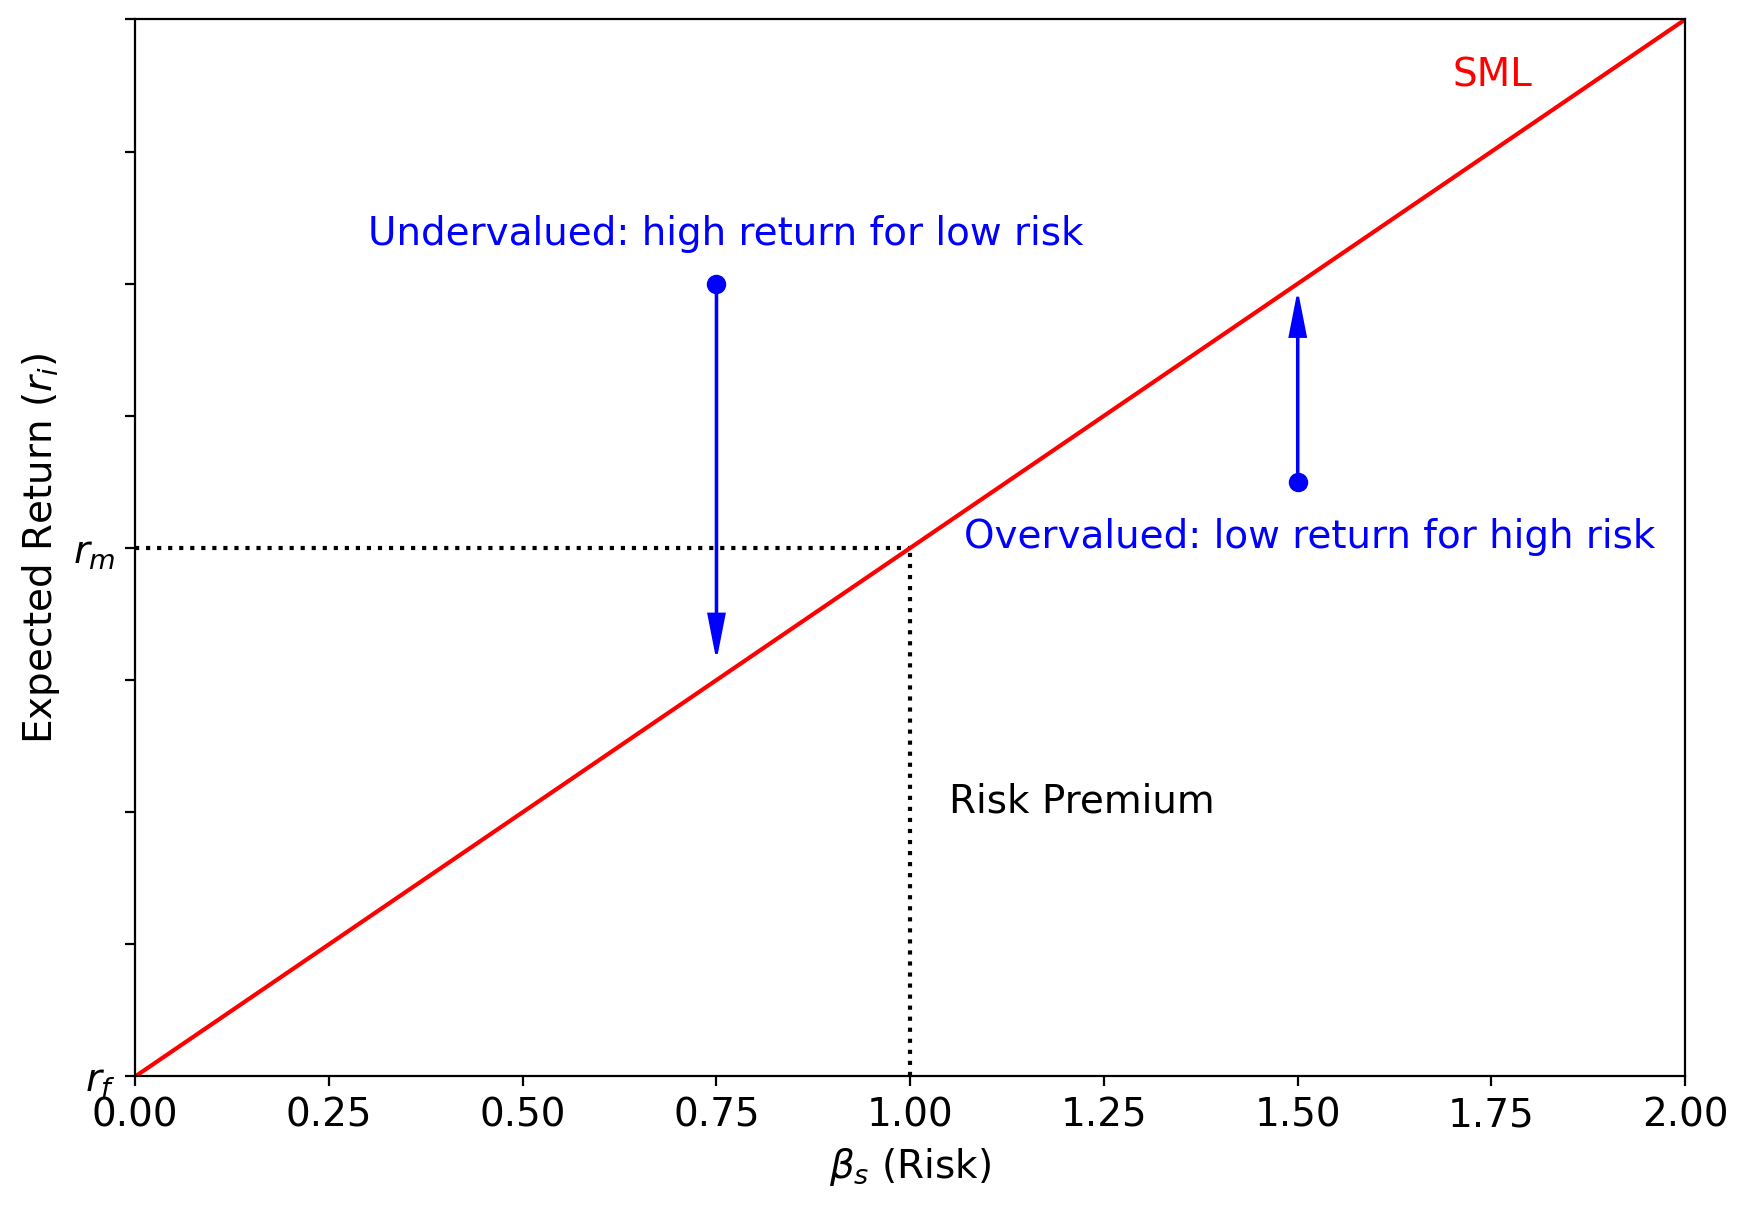
\includegraphics[width=0.7\textwidth]{figures/sml}
	\caption{Security market line.}
	\label{fig:sml}
\end{figure}

The key point in CAPM is the determination of $\beta$. This can be achieved with the measurement of the \emph{regression line} slope, in the market vs individual stock return plot.

\subsection{Regression in CAPM}

The regressed coefficient estimates can be expressed as 

\begin{equation}
	\beta \approx \cfrac{\textrm{cov}(X,y)}{\textrm {var}(X)}
\end{equation}

In the case of CAPM the line estimates the stock returns $y$ given the global market returns $X$ and so provides insights about how \emph{volatile}, or how risky, a stock is relative to the rest of the market.

In CAPM $\beta$ calculation is used to help investors understand whether a stock moves in the same direction as the rest of the market but for it to provide any useful clue, the market proxy should be related to the stock.

If $\beta$ of an individual stock = 1.0, means its price is perfectly correlated with the market, if $\beta < 1.0$, which is referred to as "defensive", indicates the security is theoretically less volatile than the market (provides lower returns, so it is less risky), while if $\beta > 1.0$, or "aggressive", indicates the assets price is more volatile than the market.

Those who use CAPM pick individual stocks or portfolios, and compare them to different indexes. The point is to find stocks that have high $\beta$, and portfolios that have high $\alpha$. High $\beta$ means the stock fares better than index with positive market and performs worse for negative market (contrary low $\beta$ gives lower performance for positive market and "better" returns in negative market), so those stocks have a chance at beating the market. $\alpha$ values above zero mean that a portfolio outperforms the market whatever it does.

\subsection{CAPM Example}

Let's apply CAPM model to a couple of securities, the market proxy is the SP500 index while the risk free rate is approximated by the 3 months Treasury rate.
Input data can be downloaded with \href{https://raw.githubusercontent.com/matteosan1/finance_course/develop/libro/input_files/capm.csv}{capm.csv}.

Consider the General Electrics (GE) stock and apply CAPM to the series of its returns. Figure~\ref{fig:ge_returns} reports the historical series of closing price for GE and SP500.

\begin{figure}[htbp]
\centering
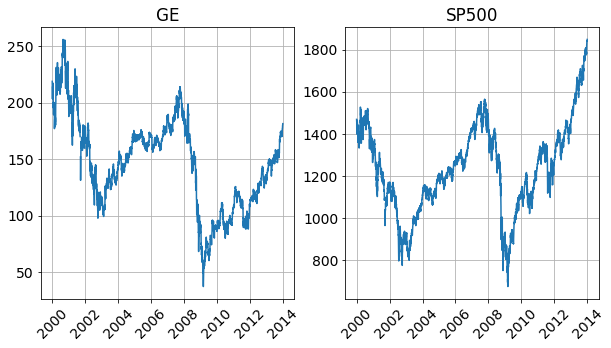
\includegraphics[width=0.7\textwidth]{figures/capm_ge}
\caption{Historical series of closing price for General Electrics stock (left) and SP500 (right).}
\label{fig:ge_returns}
\end{figure}

Using \texttt{statsmodel} it is possible to determine $\beta$ and $\alpha$ for GE stock. The model is made of GE excess of returns ($y$) and market excess of returns ($X)$ 

\begin{ipython}
X = capm['ret_SP500']
y = capm['ret_GE']

X = sm.add_constant(X)
est = sm.OLS(y, X).fit()
print(est.summary())
\end{ipython}
\begin{ioutput}
                           OLS Regression Results                                
===========================================================================
Dep. Variable:                 ret_GE   R-squared :                   0.572
Model:                            OLS   Adj. R-squared :              0.572
Method:                 Least Squares   F-statistic:                  4469.
Date:                Thu, 17 Nov 2022   Prob (F-statistic):            0.00
Time:                        08:51:58   Log-Likelihood:              9655.8
No. Observations:                3340   AIC:                     -1.931e+04
Df Residuals:                    3339   BIC:                     -1.930e+04
Df Model:                           1                                                  
Covariance Type:            nonrobust                                                  
==============================================================================
                 coef    std err          t      P>|t|      [0.025      0.975]
------------------------------------------------------------------------------
ret_SP500      1.1867      0.018     66.854      0.000       1.152       1.222
==============================================================================
Omnibus:                      900.145   Durbin-Watson:                   1.973
Prob(Omnibus):                  0.000   Jarque-Bera (JB):            66833.895
Skew:                           0.275   Prob(JB):                         0.00
Kurtosis:                      24.908   Cond. No.                         1.00
==============================================================================
\end{ioutput}

From the summary results that $\beta$ is statistically significant and equal to 1.187. Fig.~\ref{fig:capm_fit} reports the dataset and the linear regression fit.

\begin{figure}[htbp]
\centering
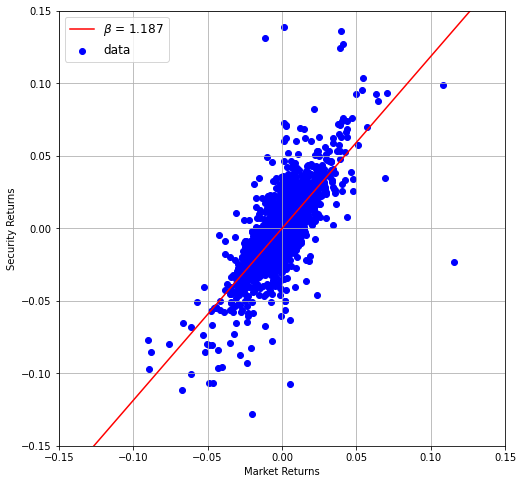
\includegraphics[width=0.7\textwidth]{figures/capm_fit}
\caption{Linear regression of market return vs stock return for GE security.}
\label{fig:capm_fit}
\end{figure}

If you imagine to have a portfolio, and that we have the $\beta$s of each individual stock to apply CAPM it is enough to perform a weighted sum of the expected return according to the model of each stock.

\subsection{Criticism to CAPM}
As we have seen the whole model is about plotting a line in a scatter plot, it’s not a very complex model. Assumptions under the model are even more simplistic. For example:
\begin{itemize}
	\tightlist
	\item expect that all investors are rational and they avoid risk;
	\item everyone have full information about the market;
	\item everyone have similar investment horizons and expectations about future movements;
	\item stocks are all correctly priced.
\end{itemize}

Moreover, this is a model from the 1960s. Market dynamics were different back then. And of course, this is a retrospective model. We cannot know how future stock prices move and how the market behaves.
Interesting extension of CAPM involves \emph{Bayesian regression}\cite{bib:bayesian_regression} but it will not be discussed here.

\section{Multifactor Models}

In its original formulation the Capital Asset Pricing Model (CAPM) treats the market return as the only factor. Nevertheless a stock’s return can depend also on other macro-economic factors, such commodity prices, interest rates, economic growth (GDP). In this case we talk about \emph{multifactor models} which can be used for: return forecasting, risk modeling, transaction cost analysis, and performance attribution. 
By decomposing asset returns into different components (\emph{factors}), allows a better understanding of the sources of portfolio return and risk. 

Factor models are based on the idea that security returns consist of two components:
\begin{itemize}
	\tightlist
\item the part that is driven by a set of common factors;
\item and the part unexplained by these factors hence idiosyncratic in nature. 
\end{itemize}
\begin{equation}
r_{t} = \sum_{k=1}^{K} X_{kt} f_{kt} + \epsilon_{t} = \mathbf{Xf} + \boldsymbol{\epsilon}
\label{eq:multifactor}
\end{equation}
where: $r_{t}$ is the security return over period $t$, $X_{kt}$ its \emph{exposure} to k$^{th}$ factor at the beginning of period $t$, $f_{kt}$ is the \emph{factor return} to k$^{th}$ factor over period $t$ and $\epsilon_{t}$ is the residual return over period $t$ (i.e. there are $K$ factors, and $T$ time periods).

\subsection{Types of Factor Models}

In practice, there are three common classes of factor models depending on the statistical techniques used to estimate factor returns and/or factor exposures.

\begin{center}
\scriptsize
\begin{tabularx}{\linewidth}{>{\hsize=.3\hsize}X>{\hsize=.4\hsize}X>{\hsize=.4\hsize}X>{\hsize=.5\hsize}X>{\arraybackslash}X}
Type & Inputs & Outputs & Estimation Method & \textcolor{ansi-green}{Adv.}/\textcolor{ansi-red}{Disadv.} \\
\toprule
Explicit & security returns, factor returns & factor exposures &\begin{tabular}[t]{@{}l@{}}time-series\\ regression\end{tabular}
		 & \textcolor{ansi-green}{Accommodates any time series as factors, linked to macroeconomic fundamentals.}
		 \textcolor{ansi-red}{Possible non-intuitive factor exposures.} \\
\midrule
Implicit & security returns, factor exposures & factor returns &\begin{tabular}[t]{@{}l@{}}cross-sectional\\ regression\end{tabular} & \textcolor{ansi-green}{Intuitive exposures linked to asset characteristics, incorporates security fundamental data, responsive to asset characteristics changes.} \textcolor{ansi-red}{Data intensive.} \\
\midrule
Statistical & security returns, factor exposures & factor returns &\begin{tabular}[t]{@{}l@{}}principal component\\analysis\end{tabular} & \textcolor{ansi-green}{Requires only asset-level price data, might capture new risk sources, relatively easy to build.} \textcolor{ansi-red}{Lack of interpretability.} \\
\end{tabularx}
\end{center}
\normalsize

\subsection{Risk Decomposition and Estimation with Factor Models}

Once factor exposures are calculated, one can carry out risk decomposition and forecast at both the individual security and the aggregate portfolio levels.

Let $R_P$ denote the return of some portfolio $P$ over period $t$
\begin{equation}
R_P = \mathbf{w}_P^T \mathbf{r}
\label{eq:portfolio_return}
\end{equation}
where $\mathbf{w}_P$ are the portfolio weights and $\mathbf{r}$ denotes the vector of security returns.

Substituting~\ref{eq:multifactor} into Eq.~\ref{eq:portfolio_return} gives
\begin{equation}
R_P = \mathbf{w}^T_P \mathbf{Xf} + \mathbf{w}^T_P\boldsymbol{\epsilon}
\end{equation}
where $\mathbf{X}$ is a $N\times K$ matrix specifying each security’s exposures to each model factors ($\mathbf{f}$). 

The risk $\sigma_P$ of the portfolio can be decomposed into the factor and the idiosyncratic components: 
\begin{equation}
\sigma^2_P = \mathbf{w}_P^T\mathbf{\Omega}\mathbf{w}_P = \mathbf{w}_P^T \mathbf{XFX}^T \mathbf{w}_P + \mathbf{w}_P^T \mathbf{\Delta} \mathbf{w}_P
\end{equation}

$\mathbf{\Omega}$ represents the $N \times N$ asset covariance matrix that without a factor model the calculation of $\mathbf{\Omega}$ would involve computing the pairwise sample covariance for each element in the matrix (e.g. $N$ is usually very large, hundreds of assets, relative to the number of time periods $T$ of the return time series, which makes the estimated covariance matrix unstable and ill-conditioned).

The factor model framework allows to reduce the dimensionality of the problem significantly. In this approach, we can express the asset covariance matrix in terms of factor model ingredients:
\begin{equation}
\mathbf{\Omega} = \mathbf{XFX}^T + \mathbf{\Delta}
\end{equation}
where $\mathbf{X}$ is the factor exposure matrix, $\mathbf{F}$ is the $K\times K$ factor covariance matrix, and $\mathbf{\Delta}$ is the $N\times N$ idiosyncratic covariance matrix (which is usually assumed to be diagonal). 

\subsubsection{Example}

Consider the example of previous Section and improve the model by adding the crude oil price as a second factor. Perform again the linear regression

\begin{ipython}
X = capm[['ret_SP500', 'ret_Brent']]
y = capm['ret_GE']

X = sm.add_constant(X)
est = sm.OLS(y, X).fit()
print(est.summary())
\end{ipython} 
\begin{ioutput}
                           OLS Regression Results                                
==============================================================================
Dep. Variable:                 ret_GE   R-squared (uncentered):          0.574
Model:                            OLS   Adj. R-squared (uncentered):     0.574
Method:                 Least Squares   F-statistic:                     2251.
Date:                Thu, 17 Nov 2022   Prob (F-statistic):               0.00
Time:                        09:05:11   Log-Likelihood:                 9662.9
No. Observations:                3340   AIC:                        -1.932e+04
Df Residuals:                    3338   BIC:                        -1.931e+04
Df Model:                           2                                                  
Covariance Type:            nonrobust                                                  
==============================================================================
                 coef    std err          t      P>|t|      [0.025      0.975]
------------------------------------------------------------------------------
ret_SP500      1.2004      0.018     66.376      0.000       1.165       1.236
ret_Brent     -0.0371      0.010     -3.768      0.000      -0.056      -0.018
==============================================================================
Omnibus:                      878.756   Durbin-Watson:                   1.974
Prob(Omnibus):                  0.000   Jarque-Bera (JB):            63119.110
Skew:                           0.231   Prob(JB):                         0.00
Kurtosis:                      24.292   Cond. No.                         1.90
==============================================================================
\end{ioutput}

The regression coefficient for the oil factor (ret\_Brent) is statistically significant and negative. Over the analysis period, price changes in GE stock are negatively related to the price changes in oil.
Let's apply the same model now to Exxon (XOM) stock.

\begin{ipython}
X = capm[['ret_SP500', 'ret_Brent']]
y = capm['ret_XOM']

X = sm.add_constant(X)
est = sm.OLS(y, X).fit()
print(est.summary())
\end{ipython} 
\begin{ioutput}
                           OLS Regression Results                                
==============================================================================
Dep. Variable:                ret_XOM   R-squared (uncentered):          0.549
Model:                            OLS   Adj. R-squared (uncentered):     0.549
Method:                 Least Squares   F-statistic:                     2031.
Date:                Thu, 17 Nov 2022   Prob (F-statistic):               0.00
Time:                        09:07:25   Log-Likelihood:                 10402.
No. Observations:                3340   AIC:                        -2.080e+04
Df Residuals:                    3338   BIC:                        -2.079e+04
Df Model:                           2                                                  
Covariance Type:            nonrobust                                                  
==============================================================================
                 coef    std err          t      P>|t|      [0.025      0.975]
------------------------------------------------------------------------------
ret_SP500      0.8129      0.014     56.082      0.000       0.785       0.841
ret_Brent      0.1453      0.008     18.391      0.000       0.130       0.161
==============================================================================
Omnibus:                      477.069   Durbin-Watson:                   2.075
Prob(Omnibus):                  0.000   Jarque-Bera (JB):             6852.309
Skew:                           0.036   Prob(JB):                         0.00
Kurtosis:                      10.017   Cond. No.                         1.90
==============================================================================
\end{ioutput}

The R-squared for XOM is slightly lower than for GE. Its relationship to the market index is less strong (lower t value).
The regression coefficient for the oil factor (ret\_Brent) is statistically significant and, unlike GE, positive.

\subsection{Fama-French Three-Factor Model}
This model was proposed in 1993 by Eugene Fama and Kenneth French to describe stock returns~\cite{bib:fama_french}. The three-factor model is
\begin{equation}
	r=\alpha + \beta_m \textrm{MKT} +\beta_s \textrm{SMB}+ \beta_h \textrm{HML}
\end{equation}
where
\begin{itemize}
	\tightlist
	\item MKT: is the excess return of the market (e.g. the value-weighted return of all firms listed on the NYSE, AMEX, or NASDAQ minus the 1-month Treasury Bill rate);
	\item SMB (Small Minus Big): measures the excess return of stocks with small market cap over those with larger market cap;
	\item HML (High Minus Low): measures the excess return of value stocks over growth stocks. Value stocks have high book to price ratio (B/P) than growth stocks.
\end{itemize}

This setting represents the original Fama-French model. This very same approach has been also extended with the Fama-French Five-Factor model which comprises two more factors:
\begin{itemize}
	\tightlist
	\item RMW (Robust Minus Weak): measures the excess returns of firms with high operating profit margins over those with lower profits;
	\item CMA (Conservative Minus Aggressive): measures the excess returns of firms investing less over those investing more.
\end{itemize}
Finally, momentum is another commonly used factor. It captures excess returns of stocks with highest returns over those with lowest returns.

The application of such models goes along the lines of the CAPM with the only difference being the calculation of a multidimensional regression.

%* The Fama and French model has three factors: 
%* the size of firms (**SMB**, small minus big), 
%* book-to-market values (**HML**, high minus low), 
%* **excess return on the market** (portfolio's return less the risk-free rate of return). 
%
%* SMB accounts for publicly traded companies with small market caps that generate higher returns, while HML accounts for value stocks with high book-to-market ratios that generate higher returns in comparison to the market.
%
%* Represent each characteristic of interest ($f_k(t)$) by a portfolio: 
%1. sort all assets by that characteristic;
%2. build the portfolio by going long the top quantile of assets and short the bottom quantile. 
%
%* **The factor corresponding to this characteristic is the return on this portfolio**. 
%* The $X_{nk}(t)$ are estimated for each asset $n$ by regressing over the historical values of $r_n(t)$ and of the factors.


\section*{Exercises}

\cprotEnv\begin{question}
The Dow-Jones Industrial Average (DJIA) was first introduced by Charles Dow in 1896 and has since become one of the main references for stock market performance on the New York Stock Exchange.

In this post, we will use it to better understand the pros and cons of simple Linear Regression models, the assumptions they rely on, and how we can use them for feature selection.

Its value is determined with a weighted average of 30 stock prices. Since the Dow components change over time, using the provided dataset (\href{"https://github.com/matteosan1/finance_course/raw/master/input_files/dji.csv}{dji.csv}) and a list of 35 assets, determine which of them are included in the calculation given a time interval. Try to interpret the results.

\textbf{Hint}: in order to cross-check your result split the dataset in two parts (before and after August 2020), then fit the model with the first part and test it with the second.
\begin{ipython}
selected = ['AAPL', 'AMGN', 'AXP', 'BA', 'CAT', 'CRM', 'CSCO', 'CVX', 'DD', 'DIS', 
            'DOW', 'GE', 'GS', 'HD', 'HON', 'IBM', 'INTC', 'JNJ', 'JPM', 'KO', 'MCD', 
            'MMM', 'MRK', 'MSFT', 'NKE', 'PFE', 'PG', 'RTX', 'TRV', 'UNH', 'V', 'VZ', 
            'WBA', 'WMT', 'XOM']
\end{ipython}
\end{question}

\cprotEnv\begin{solution}
Load the dataset and split into two dataframes DJI and the other tickers.
\begin{ipython}
import pandas as pd

closing = pd.read_csv("dji.csv", index_col='Date')
DJI = closing['DJI'].copy()
closing.drop(columns='DJI', inplace=True)
\end{ipython} 
	
\begin{figure}[htbp]
\centering
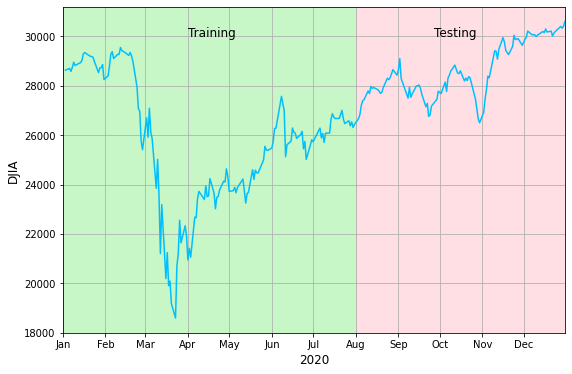
\includegraphics[width=0.7\textwidth]{figures/dji}
\caption{DJIA index daily values in 2020. The dataset has been divided into two parts for training and testing purpose.}
\label{fig:dji-returns}
\end{figure}
	
We need to fit the linear model to the available data prior to August 2020 (\emph{notice that the dataset already contains the intercept column to take care of the $\alpha$ parameter}), see Fig.~/ref{fig:dji-returns}.
\begin{ipython}
import statsmodels.api as sm

model = sm.OLS(DJI[DJI.index <='2020-07-31'], 
               closing[closing.index <='2020-07-31']).fit()
print (model.summary())
\end{ipython}
\begin{ioutput}
                          OLS Regression Results                            
==============================================================================
Dep. Variable:                    DJI   R-squared:                       1.000
Model:                            OLS   Adj. R-squared:                  1.000
Method:                 Least Squares   F-statistic:                 2.107e+06
Date:                Tue, 08 Nov 2022   Prob (F-statistic):          1.99e-297
Time:                        18:16:13   Log-Likelihood:                -364.32
No. Observations:                 143   AIC:                             800.6
Df Residuals:                     107   BIC:                             907.3
Df Model:                          35                                         
Covariance Type:            nonrobust                                         
==============================================================================
coef    std err          t      P>|t|      [0.025      0.975]
------------------------------------------------------------------------------
AAPL          28.1315      0.238    118.405      0.000      27.660      28.602
AMGN           0.0701      0.098      0.714      0.477      -0.124       0.265
AXP            6.2508      0.261     23.940      0.000       5.733       6.768
BA             7.0296      0.047    149.349      0.000       6.936       7.123
CAT            6.8530      0.160     42.953      0.000       6.537       7.169
CRM            0.0452      0.123      0.367      0.714      -0.199       0.289
CSCO           6.9258      0.564     12.274      0.000       5.807       8.044
CVX            7.6117      0.260     29.233      0.000       7.096       8.128
DD             0.4722      0.318      1.484      0.141      -0.159       1.103
DIS            6.9450      0.178     39.057      0.000       6.593       7.298
DOW            6.3940      0.387     16.541      0.000       5.628       7.160
GE             0.2437      0.216      1.130      0.261      -0.184       0.671
GS             6.9331      0.122     56.636      0.000       6.690       7.176
HD             6.6309      0.096     69.009      0.000       6.440       6.821
HON           -0.3708      0.193     -1.918      0.058      -0.754       0.012
IBM            7.3397      0.202     36.317      0.000       6.939       7.740
INTC           6.5288      0.199     32.789      0.000       6.134       6.924
JNJ            6.7114      0.240     27.962      0.000       6.236       7.187
JPM            6.7418      0.236     28.578      0.000       6.274       7.209
KO             6.9641      0.572     12.173      0.000       5.830       8.098
MCD            6.8349      0.150     45.446      0.000       6.537       7.133
MMM            6.4935      0.146     44.401      0.000       6.204       6.783
MRK            7.5556      0.318     23.792      0.000       6.926       8.185
MSFT           6.4336      0.155     41.509      0.000       6.126       6.741
NKE            6.7713      0.231     29.369      0.000       6.314       7.228
PFE            8.0045      0.466     17.163      0.000       7.080       8.929
PG             7.0308      0.294     23.894      0.000       6.447       7.614
RTX            8.4790      0.301     28.136      0.000       7.882       9.076
TRV            6.7275      0.194     34.767      0.000       6.344       7.111
UNH            6.7560      0.073     93.183      0.000       6.612       6.900
V              7.2610      0.174     41.824      0.000       6.917       7.605
VZ             6.6514      0.631     10.546      0.000       5.401       7.902
WBA            6.2044      0.331     18.750      0.000       5.548       6.860
WMT            6.7940      0.211     32.258      0.000       6.376       7.212
XOM            6.0549      0.487     12.435      0.000       5.090       7.020
intercept     -4.1082     21.263     -0.193      0.847     -46.259      38.043
==============================================================================
Omnibus:                       19.720   Durbin-Watson:                   2.012
Prob(Omnibus):                  0.000   Jarque-Bera (JB):               62.557
Skew:                          -0.398   Prob(JB):                     2.61e-14
Kurtosis:                       6.141   Cond. No.                     5.70e+04
==============================================================================
\end{ioutput}

From the $p$-values in Figure~\ref{fig:p-values} (left), we can quickly identify the stocks whose weights are not meaningfully different from zero, namely: AMGN, CRM, DD, GE, and HON. The reason is simply that they are not part of the DJIA in the considered period.
Repeating the fit with the updated model shows that all the included tickers are still contributing to the DJIA index determination, see Fig.~\ref{fig:p-values} (right).
	
\begin{ipython}
selected_columns = list(model.pvalues[model.pvalues<0.05].index)

model_small = sm.OLS(DJI[DJI.index <= '2020-07-31'], 
                     closing[selected_columns][closing.index <= '2020-07-31']).fit()
print (model_small.summary())
\end{ipython}
\begin{ioutput}
                        OLS Regression Results                                
==============================================================================
Dep. Variable:                    DJI   R-squared (uncentered):          1.000
Model:                            OLS   Adj. R-squared (uncentered):     1.000
Method:                 Least Squares   F-statistic:                 2.434e+08
Date:                Thu, 26 Jan 2023   Prob (F-statistic):               0.00
Time:                        11:59:44   Log-Likelihood:                -369.56
No. Observations:                 143   AIC:                             799.1
Df Residuals:                     113   BIC:                             888.0
Df Model:                          30                                                  
Covariance Type:            nonrobust                                                  
==============================================================================
                 coef    std err          t      P>|t|      [0.025      0.975]
------------------------------------------------------------------------------
AAPL          28.1695      0.229    123.120      0.000      27.716      28.623
AXP            6.2176      0.250     24.878      0.000       5.722       6.713
BA             7.0379      0.045    157.710      0.000       6.949       7.126
CAT            6.7754      0.133     50.871      0.000       6.511       7.039
CSCO           7.2883      0.535     13.620      0.000       6.228       8.348
CVX            7.5201      0.239     31.522      0.000       7.047       7.993
DIS            6.8027      0.163     41.760      0.000       6.480       7.125
DOW            6.6917      0.338     19.793      0.000       6.022       7.361
GS             6.9423      0.116     59.693      0.000       6.712       7.173
HD             6.6851      0.089     75.149      0.000       6.509       6.861
IBM            7.2860      0.196     37.126      0.000       6.897       7.675
INTC           6.4310      0.189     34.007      0.000       6.056       6.806
JNJ            6.7935      0.215     31.583      0.000       6.367       7.220
JPM            6.8400      0.214     31.945      0.000       6.416       7.264
KO             6.5188      0.494     13.206      0.000       5.541       7.497
MCD            6.7657      0.139     48.518      0.000       6.489       7.042
MMM            6.4385      0.121     53.174      0.000       6.199       6.678
MRK            7.5965      0.296     25.622      0.000       7.009       8.184
MSFT           6.5577      0.134     48.935      0.000       6.292       6.823
NKE            6.7307      0.208     32.385      0.000       6.319       7.142
PFE            8.0817      0.454     17.806      0.000       7.182       8.981
PG             6.9862      0.267     26.144      0.000       6.457       7.516
RTX            8.6628      0.275     31.476      0.000       8.118       9.208
TRV            6.5894      0.181     36.417      0.000       6.231       6.948
UNH            6.6966      0.066    100.982      0.000       6.565       6.828
V              7.2778      0.160     45.487      0.000       6.961       7.595
VZ             6.3851      0.526     12.134      0.000       5.343       7.428
WBA            6.2725      0.304     20.631      0.000       5.670       6.875
WMT            6.9055      0.198     34.832      0.000       6.513       7.298
XOM            6.5498      0.443     14.782      0.000       5.672       7.428
==============================================================================
Omnibus:                       27.413   Durbin-Watson:                   1.905
Prob(Omnibus):                  0.000   Jarque-Bera (JB):               91.998
Skew:                          -0.630   Prob(JB):                     1.05e-20
Kurtosis:                       6.722   Cond. No.                     1.70e+03
==============================================================================
\end{ioutput}
\begin{figure}[htbp]
\centering
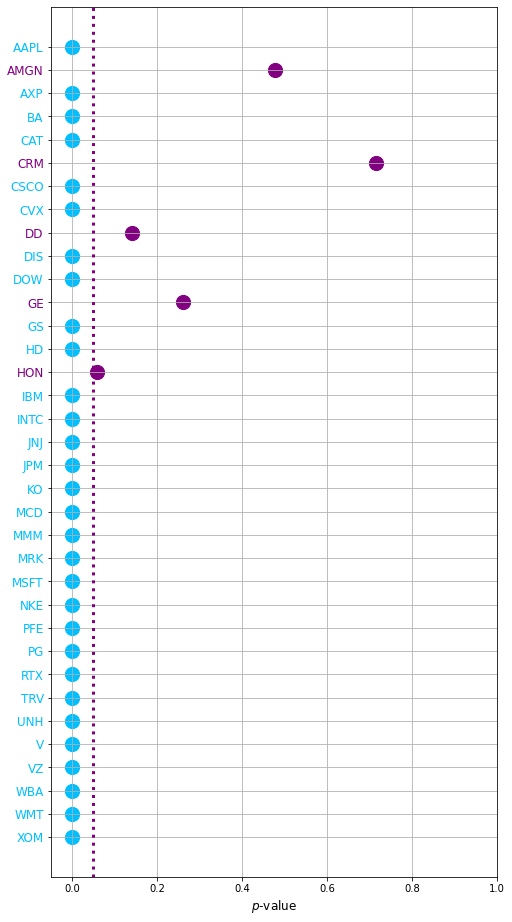
\includegraphics[width=0.4\textwidth]{figures/p-values}
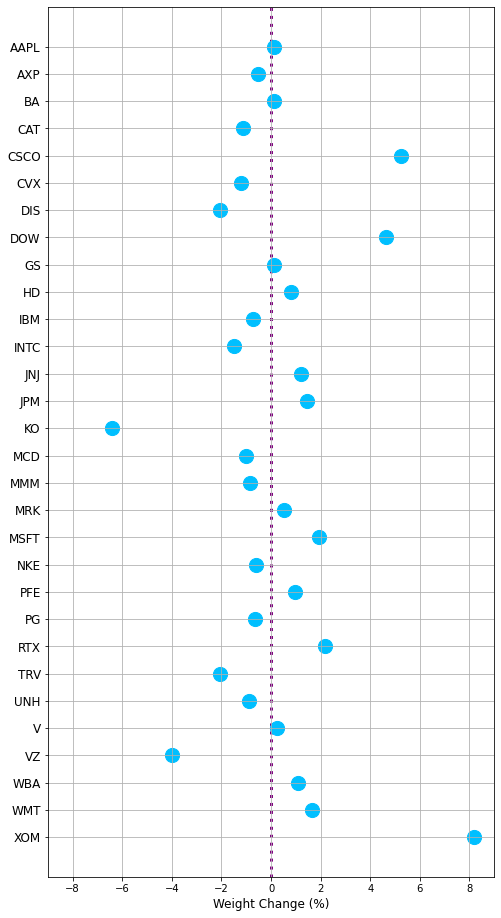
\includegraphics[width=0.4\textwidth]{figures/delta_weights}
\caption{$p$-values resulting from the linear model fit to DJIA returns (left). Parameter percentage difference according to the two models described in the text (right).}
\label{fig:p-values}
\end{figure}
	
Now that we have a good model it is possible to check how it behaves on the test sample (i.e. from August to December 2020). The result is shown in Figure~\ref{fig:prediction}. The residuals plot, the difference between predicted and actual values of the DJIA, shows that there is a clear degradation of the performance after September, see Fig.~\ref{fig:residuals}.

\begin{ipython}
residuals = DJI-model_small.predict(closing[selected_columns])
\end{ipython}
	
\begin{figure}[htbp]
\centering
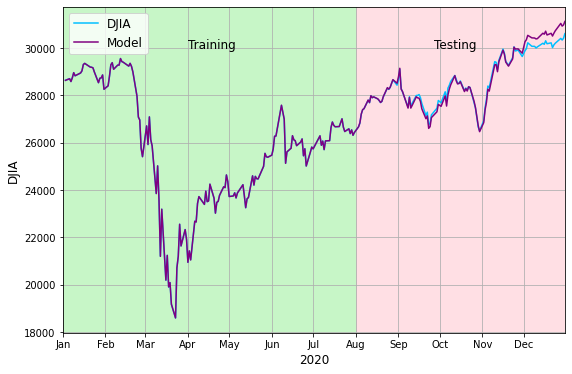
\includegraphics[width=0.7\textwidth]{figures/prediction}
\caption{Model prediction to DJIA index performance comparison.}
\label{fig:prediction}
\end{figure}

As we can see, our model works extremely well for the first few weeks of the testing period and then it completely falls apart. The reason for this puzzling behavior is surprisingly simple: the fundamental assumption underlying our model was no longer valid. The \textbf{composition of the DJIA changed on Aug 31st, 2020} with Pfizer, Raytheon, and Exxon Mobile being dropped and replaced by Amgen, Honeywell, and Salesforce.

\begin{figure}[htbp]
\centering
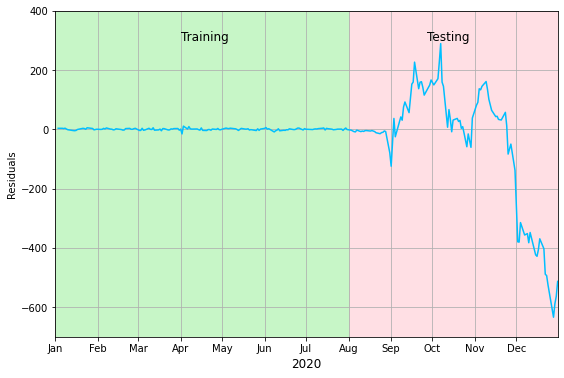
\includegraphics[width=0.7\textwidth]{figures/residuals}
\caption{Residuals of the linear model.}
\label{fig:residuals}
\end{figure}
\end{solution}

\begin{question}
Stock A has a $\beta$ of 1.2 and Stock B has a $\beta$ of 0.6. Which of the following statements is true? 
\begin{enumerate}[label=\emph{\alph*})]
\tightlist
\item Stock A has more unsystematic risk than Stock B;
\item Stock B has more systematic risk than Stock A; 
\item if the risk-free rate and the market risk premium are both positive, Stock A has a higher expected return than Stock B according to the CAPM;
\item both \emph{a} and \emph{b} are true;
\item both \emph{b} and \emph{c} are true
\end{enumerate}
\end{question}

\begin{solution}
The correct answer is \emph{c} indeed according to CAPM formula
\[r_i = r_f + \beta_i (r_M - r_f)\]
if both $r_f$ and $(r_M - r_f)$ are positive then $r_A > r_B$.
\end{solution}	

\begin{question}
Consider a stock with a $\beta$ of 1.5. Which of the following statements is true?

\begin{enumerate}[label=\emph{\alph*}]
\tightlist
\item when the market goes down by 1.5\%, on average, the stock goes down by 1\%;
\item when the market goes up by 1.5\%, on average, the stock goes up by 1\%;
\item when the market goes up by 1\%, on average, the stock goes down by 1.5\%;
\item when the market goes down by 1\%, on average, the stock goes down by 1.5\%. 
\item both \emph{a} and \emph{b}.	
\end{enumerate}
\end{question}

\begin{solution}
The correct answer is \emph{d} since $\beta$ measures the slope of the regression line of the expected return of the stock vs the expected return of the market. So by definition it represents the variation of the stock expected return given the a unit variation of the expected return of the market.
\end{solution}	

\begin{question}
Suppose that the risk-free rate is 3\% and the market risk premium is 8\%. According to the CAPM, what is the required rate of return on a stock with a $\beta$ of 2 ?
\end{question}

\begin{solution}
Careful! The market risk premium is 8\%. This means that $r_M - r_f  = 8\%$. Plug this into the CAPM equation to get

\begin{equation*}
r = r_f + \beta(r_M - r_f) = 3\% + 2\cdot(8\%) =19\%
\end{equation*}
\end{solution}

\begin{question}
You analyze the prospects of several companies and come to the following conclusions about the required return on each:

\begin{center}
\begin{tabular}{lc}
\textbf{Stock Required} & \textbf{Return} \\
Starbucks &18\% \\
Sears &8\% \\
Microsoft &16\% \\
Limited Brands &12\% \\
\end{tabular}
\end{center}

You decide to invest \$4000 in Starbucks, \$6000 in Sears, \$12000 in Microsoft, and \$3000 in Limited Brands. What is the required return on your portfolio?
\end{question}

\cprotEnv \begin{solution}
\begin{ipython}
P = 4000 + 6000 + 12000 + 3000
rp =(4000/P)*0.18 + (6000/P)*0.08 + (12000/P)*0.16 +(3000/P)*0.12
print (f"Portfolio Return: {rp*100:.2f}%")
\end{ipython}
\begin{ioutput}
Portfolio Return: 13.92%
\end{ioutput}
\end{solution}	

\begin{question}
You have a portfolio that consists of 35\% Microsoft stock, 35\% Amazon stock, and 30\% GE stock. Microsoft has a $\beta$ of 1, Amazon has a $\beta$ of 3.0, and GE has a $\beta$ of 0.5. Treasury bills (the risk-free asset) currently offer a return of 4\%, and the expected return on the market is 11.5\%. What return should you expect on your portfolio according to the CAPM ? 
\end{question}

\cprotEnv \begin{solution}
You can work this problem two different ways.

\textbf{Method 1}: calculate the $\beta$ of your portfolio and plug this $\beta$ into the CAPM formula to get the required return of your portfolio.

\begin{ipython}
rm = 0.115
rf = 0.04
beta_p = 0.35 * 1 + 0.35 * 3 + 0.3 * 0.5
rp = rf + beta_p*(rm - rf)

print (f"Portfolio beta: {beta_p:.2f}")
print (f"Portfolio return: {rp*100:.3f}%")
\end{ipython}
\begin{ioutput}
Portfolio beta: 1.55
Portfolio return: 15.625%
\end{ioutput}

\textbf{Method 2}: using the CAPM, calculate the required return on each individual stock. Then,calculate the weighted average of those required returns to get the required return of your portfolio.

\begin{ipython}
Er_msft = rf + 1*(rm-rf)
Er_amzn = rf + 3*(rm-rf)
Er_ge = rf + 0.5*(rm-rf)
rp2 = Er_msft * 0.35 + Er_amzn *0.35 + Er_ge * 0.3

print (f"Er (MSFT): {Er_msft*100:.2f}%")
print (f"Er (AMZN): {Er_amzn*100:.2f}%")
print (f"Er (GE): {Er_ge*100:.2f}%")
print (f"Portfolio return: {rp2*100:.3f}%")
\end{ipython}
\begin{ioutput}
Er (MSFT): 11.50%
Er (AMZN): 26.50%
Er (GE): 7.75%
Portfolio return: 15.625%
\end{ioutput}
Notice that this is the same answer we got using method 1. When calculating the required return of a portfolio, it does not matter which way you do it. But method 1 is a little less work.
\end{solution}


\begin{thebibliography}{9}
\bibitem{bib:bayesian_regression}W. Kohersen, \href{https://towardsdatascience.com/introduction-to-bayesian-linear-regression-e66e60791ea7}{\emph{Introduction to Bayesian Linear Regression}}, Toward Data Science [Online]
\bibitem{bib:fred}\href{https://fred.stlouisfed.org/}{\emph{FRED Economic data}}, 1991 [Online]
\bibitem{bib:capm_lintner} Lintner, J. \emph{“The Valuation of Risky Assets and the Selection of Risky Investments in Stock Portfolio and Capital Budgets}, 1965, Review of Economics and
Statistics, 47: 13-37.
\bibitem{bib:capm_sharpe} Sharpe, W. \emph{Capital Asset Prices: A Theory of Market Equilibrium under Conditions of Risk}, 1964, Journal of Finance, 19: 425-442.
\bibitem{bib:fama_french} E. F. Fama, K. R. French \emph{Common risk factors in the returns on stocks and bonds}, Journal of Financial Economics, 1993, doi:10.1016/0304-405X(93)
\end{thebibliography}



